\documentclass[facebook_diary.tex]{subfiles}

\begin{document}

\chapter{2022年}

\section{4月}

\subsection*{2022年04月23日 14:18}
\addcontentsline{toc}{subsection}{2022年04月23日 14:18}

この指揮(者)面白すぎる!

指示がとても細かいので、スコアを見ながら聞きたいほどだ。

ハープのアルペジオの扱いはとてもユニーク。

(弦のピッツは入っているのかどうか？分からないけど)

アインザッツの一つ一つが決まっている。消音の指示も細かい。

旋律的な部分ではゆったりと弦に十分歌わせている。

たっぷりのsfのようなディナーミクも素敵だ。

終わりの方へ行くにつれて指揮がまるで踊りの様になっていく。

装飾音の様な音形の所では身を捩らせて表現している。

所々で「歌舞伎の見得」の様なストップモーションが入る。

ラッパの音と一緒に「パパパパーン、パーン」と歌いながら踊っている。本当に、Too funny‼︎ だ。(一番最後の音はもっと短いものとの予断を持っていたのだが)

\paragraph{リンク}
\url{https://youtube.com/watch?v=vnj3K3jaUV4&feature=share}

\subsection*{2022年04月23日 16:37}
\addcontentsline{toc}{subsection}{2022年04月23日 16:37}

3月24日に子供2人が(同日に)大学院(修士と博士)を修了しました。

コロナ禍のため家族は式場に入れません。下の子は校門前での撮影も禁止だという話でした(\url{http://www.nara-wu.ac.jp/nwu/news/2021news/20220324.html})が、写真撮影の順番を待つ列ができていました。また、上の子の方は式の様子がYoutubeで配信(\url{https://youtu.be/_U3jf54yJQI?t=2917})されていました。

2人ともそれぞれの専門を活かして、社会で元気に活躍していってくれる事を願っています。

\paragraph{写真}
\begin{center}
\begin{minipage}{0.70\linewidth}
\centering
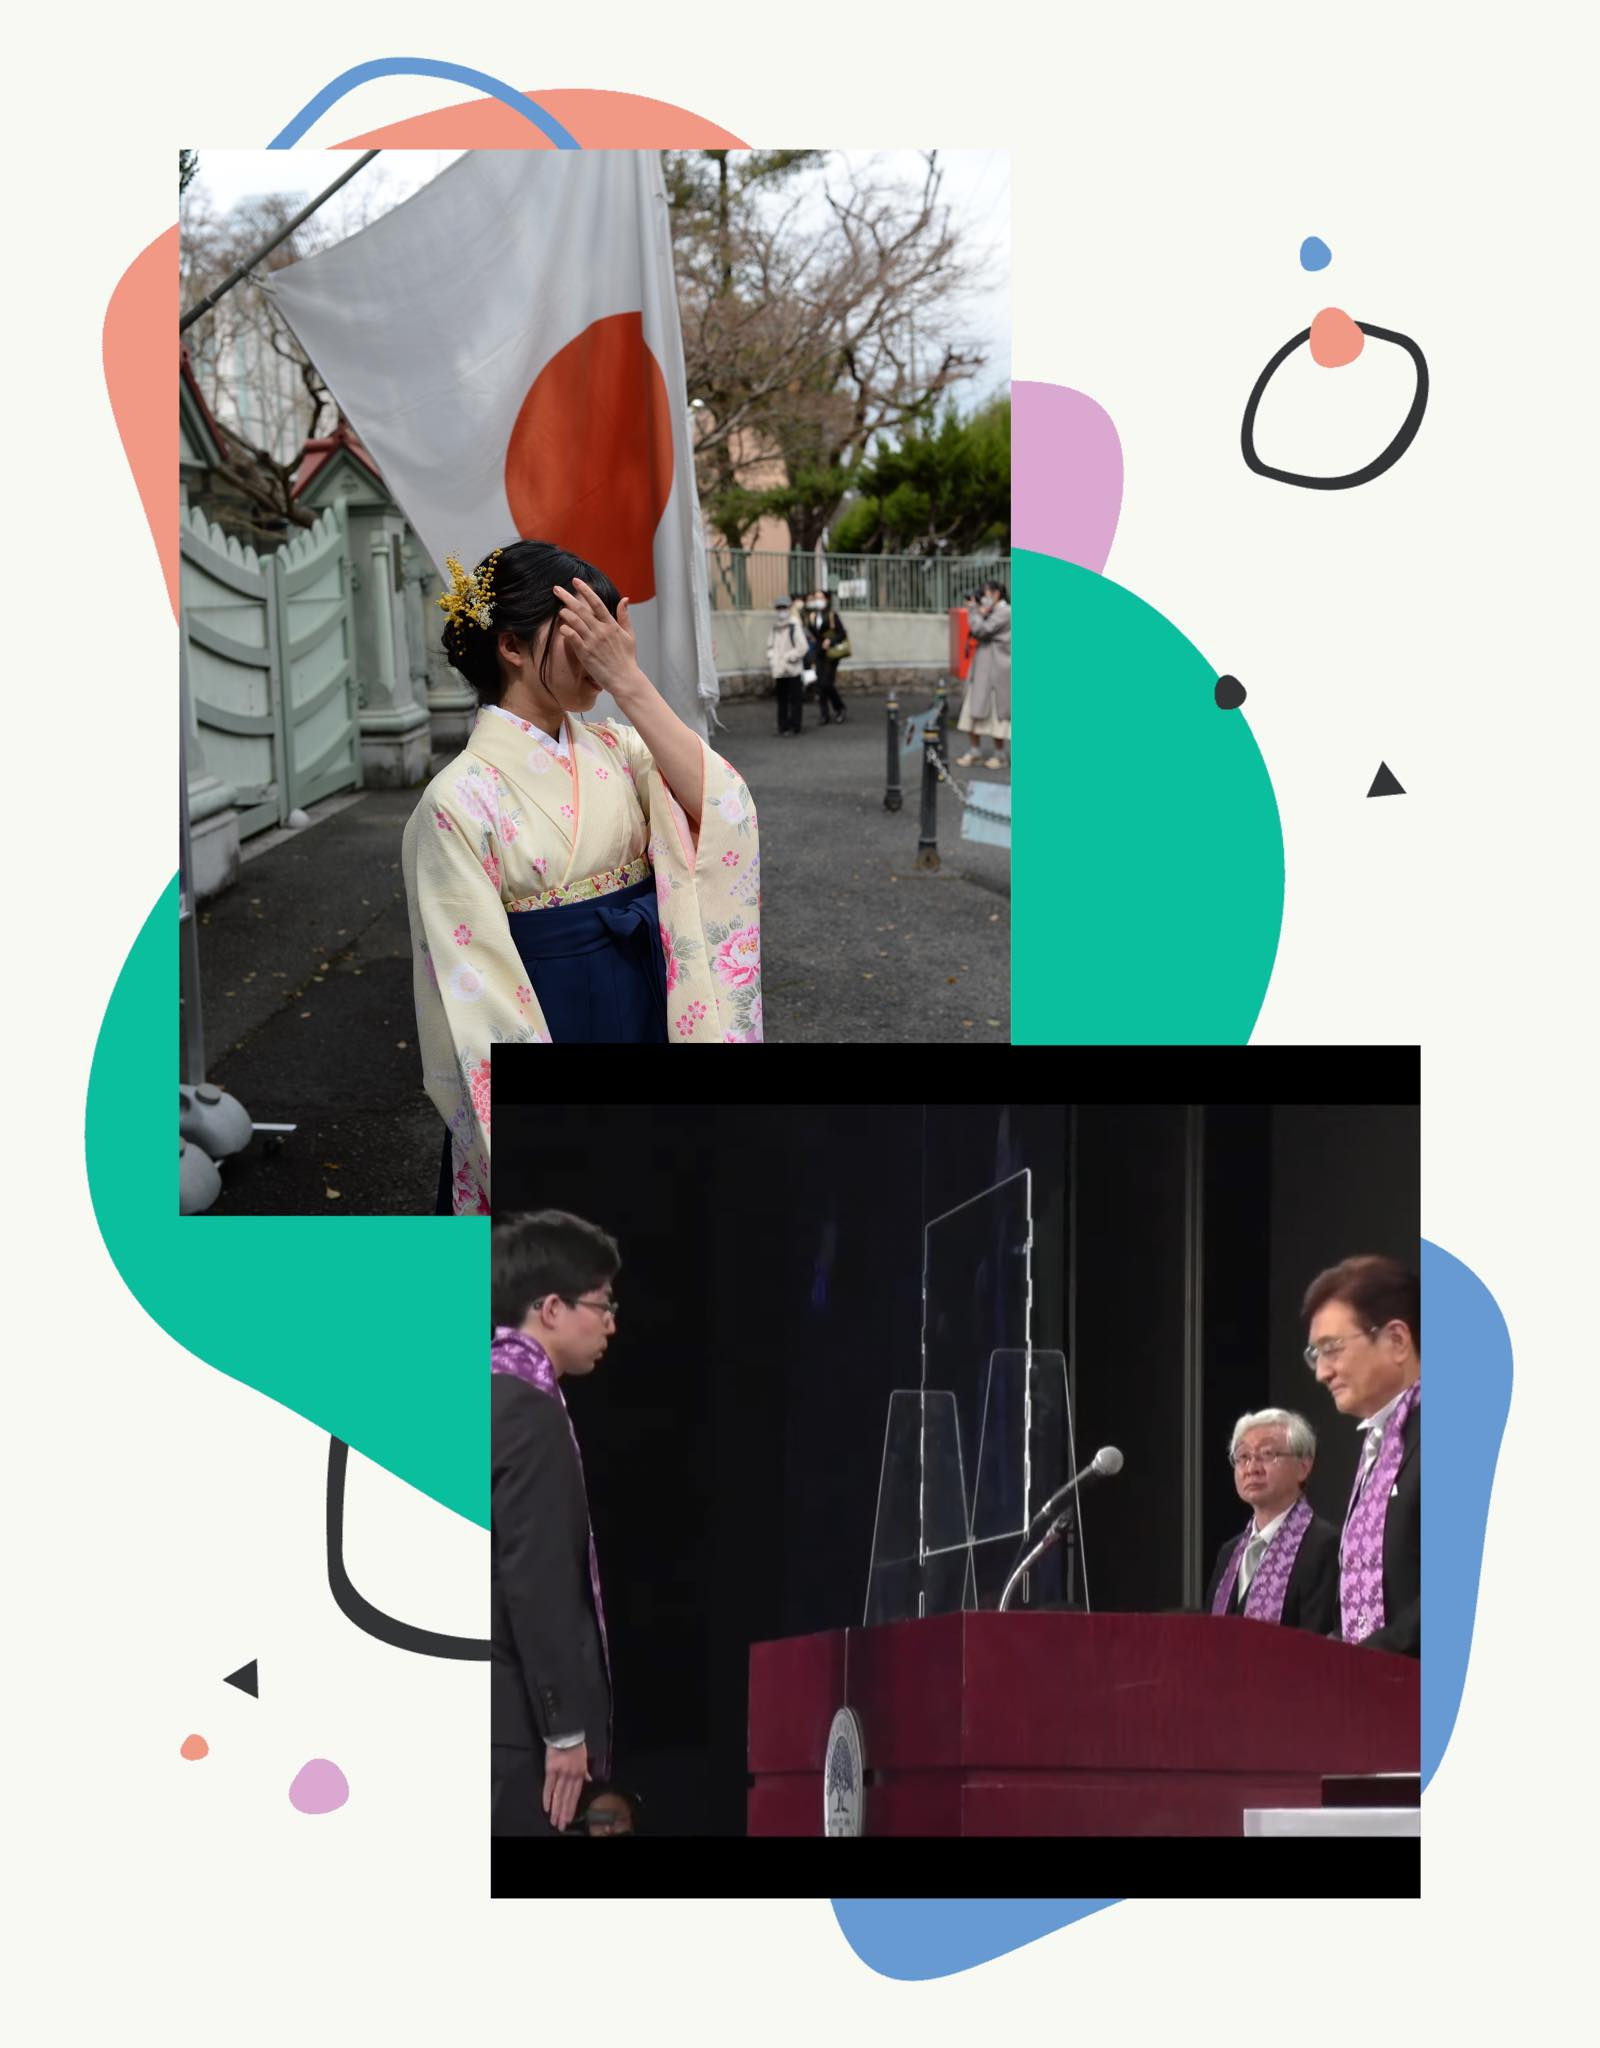
\includegraphics[width=\linewidth]{pictures/2022/04/20220423_163737_001.jpg}
\end{minipage}
\end{center}

\subsection*{2022年04月24日 17:23}
\addcontentsline{toc}{subsection}{2022年04月24日 17:23}

ここは京都伏見にある明治天皇の桃山御陵です。

単に重力に抗してする仕事の動画です。

ただただハアハア言っているだけのことなので、全部見る人はいないと思いますが、さてこの階段は何段あるでしょうか？

登る時は数える余裕はなかったのですが、降りる時に数えてきました。23段毎に踊り場があって、それが10個連なっているので全部で230段です。途中まで登ってきたら、ここから降りるというのも無駄なことをしたという気になると思い、無理やり1番上まで登りました。

帰りにちょうど登り口に差し掛かったアベックに出会いました。女性の方が「私は絶対無理」と言って引き返そうとしていて、男性の方が「それじゃあ写真だけ撮ろう」と言ってなだめていました。

\paragraph{リンク}
\url{https://youtube.com/watch?v=_YPzNmcYFTw&feature=share}

\section{10月}

\subsection*{2022年10月06日 21:15}
\addcontentsline{toc}{subsection}{2022年10月06日 21:15}

核融合が実用になる頃には、もうこの世にいないだろうなぁ。

\section{11月}

\subsection*{2022年11月11日 22:09}
\addcontentsline{toc}{subsection}{2022年11月11日 22:09}

\url{https://youtu.be/UsI7xwRgSfM}

素敵な演奏です。

最初冷静に歌われているけれども、同じテーマが少しづつ気持ちの昂りを語る様になり、ピアノと一緒にテーマを鳴らしてからは、後半繰り返し押し寄せる慟哭を聞かされる様です。最後には大きな波が引いて静かな凪が戻った様に、諦観にも聞こえます。

曲想を編曲、演奏を通して効果的に聴き手に伝えることに成功していると思います。

\paragraph{リンク}
\url{https://youtu.be/UsI7xwRgSfM}

\subsection*{2022年11月12日 23:07}
\addcontentsline{toc}{subsection}{2022年11月12日 23:07}

\url{https://youtu.be/x6fe52vi_ME}

ごまかしのない、丁寧で素直な表現、優しい演奏が印象的です。

重厚な弦のたっぷり歌わせるアウフタクト、ピッツの音、シンコペ、付点のリズム、ホルンの丸い響き、あれもこれも最初から最後まで、あーブラームスだなと感じさせてくれます。コンミスのソロは勿論のこと、木管のソロもそれぞれとても美しく、一生懸命練習して臨んでいるんだろうなと思うと涙がこぼれそうになります。

\paragraph{リンク}
\url{https://youtu.be/x6fe52vi_ME}

\subsection*{2022年11月17日 00:59}
\addcontentsline{toc}{subsection}{2022年11月17日 00:59}

\url{https://youtu.be/oqh2k_5Ido4}

フルート吹きならみんな好きな曲です。

（A=415Hzの様です。トラヴェルソによる演奏かな）

この映像表現は面白い。

曲を演奏する時の、言うならば、

「アーティキュレーションを絵に描いたよう」

にも見えてきます。

\paragraph{リンク}
\url{https://youtu.be/oqh2k_5Ido4}

\subsection*{2022年11月17日 08:01}
\addcontentsline{toc}{subsection}{2022年11月17日 08:01}

\url{https://youtu.be/y0CCCWlDIPM}

こんな「お話」だったのか。（詳しく知りませんでした）

ソロイストの皆さんがとても上手なので、最後まで引き込まれます。

（ビオラが一カ所音外している様な気もするけど）

この曲は個人的には思い出深い曲です。

学生の頃にこの曲と出会う事ができて、

この曲と比較的深く関われた事を思い出しては、

本当に良かったなと思います。

\paragraph{リンク}
\url{https://youtu.be/y0CCCWlDIPM}

\subsection*{2022年11月17日 23:28}
\addcontentsline{toc}{subsection}{2022年11月17日 23:28}

\url{https://youtu.be/GX2EFYL_LOM}

フィガロの序曲を一人で演奏している。

この方とってもお上手です。

指の動きは素早いし、こんなにも速いタンギング、私には到底できる様になるとは思えません。trtrt,trtrtrtrtrtrtかな。（どうやって録音したのか。一番最初に録音したのはどのパートだろうか。録音機材も含めて実は気になっています）

学生の頃にカール・ベームとウイーン国立歌劇場管弦楽団が来日し、フィガロが上演されました。当時NHKのTVを見ただけなのですが、フィガロを聞いた最初の出来事です。

スザンナを歌ったのはルチア・ポップ。ケルビーノはフレデリカ・フォン・シュターデだったか（アグネス・バルツァだったのか？）とにかく、とてもチャーミングだったので直ぐにファンになりました。

また、ベームの指揮が、あまり動かずに、ぶるぶるっと震える様な仕草だったので、オケの方はどうやって合わせているんだろうと不思議に思った記憶があります。（みんなコンマスに合わせているという説を聞いた事がありますが、真偽の程は不明です）

ワーグナーの楽劇何某をジッと見ている時間があるなら、その時間はフィガロや魔笛を繰り返し聞いている方が、ずっと幸せな人生の時間を過ごす事ができると言うのが私の持論です。

\paragraph{リンク}
\url{https://youtu.be/GX2EFYL_LOM}

\subsection*{2022年11月18日 07:23}
\addcontentsline{toc}{subsection}{2022年11月18日 07:23}

\url{https://youtu.be/L2DxxblM_Es}

これ、実は大好きな曲なのです。

各声部（パート）のリズムがとても複雑であるにも拘らず、曲全体として紛れもなくワルツであると感じます。ワルツに合わせて体が動いて踊ってしまいます。またオーケストラ版では、いろいろな楽器の音の重ね合わせなどに、オーケストレーションの神様モーリス・ラベルの天才を感じずにはいられません。

「音」を聞いて「色」が見えることって、ありますか？

教養の時の心理学の講義で、年老いた先生（足が少し不自由な様子でした）が、指を舐めては古いノートのページをめくりながら（何年も使っていらっしゃるノートらしく、ノートの右下の角が少しめくれていました）話されていたのを、なぜか今でもその時のことを鮮やかに思い出します。「音を聞くと色が見えるっていう人がいるらしいんだ」こんなゆっくりとした口調で話されていました。「へーそんな人いるの？自分には感じられんな」と思っていました。ところが、エルネスト・アンセルメ-スイス・ロマンド（だったか？）のレコードを聞いた時に、曲の終わりの方でハープのグリッサンド？が上下降するのに重ねて、スフォルツァンドの様な弦の音（管もユニゾンだね、きっと）のうねりが繰り返される部分辺りから「パレットの上の絵の具を全部一気にひっくり返した様な」（何処かでこんな表現に出会った事があった様な気がします）様々な色を感じた気がしました。「どの音が何色」とかではなく「たくさんの色が一気に」です。いろんな色の絵の具がチューブから飛び出してくる、あるいは水面をたくさんの色が混沌と漂って動いている（決して渦の様な綺麗な形をした動きではなくて）、画板上を乱暴に塗りたくられた油絵の具の、いや、水彩かもしれません、それらの言わばChaosなイメージを感じます。

こちらは演奏している映像

2003年

\url{https://youtu.be/hkVrhll9VBA}

緊迫の、息を飲む演奏です

1982年

\url{https://youtu.be/mwBuhTZtDT0}

この２つの演奏を最後まで見ると、アルへリッチが20年の齢を重ねて丸くなっている様な気がします。（譜めくリストって誰でもできる様な役目ではないですね。大変だ。）

\paragraph{リンク}
\url{https://youtu.be/L2DxxblM_Es}

\subsection*{2022年11月18日 16:51}
\addcontentsline{toc}{subsection}{2022年11月18日 16:51}

\url{https://youtu.be/sJU5aGNUahU}

やっぱり若者の演奏はいいです。

純粋で清々しい。聞く方もそんな気持ちになります。

懐かしさを感じさせる武満の曲と相まって、本当に心が洗われるようです。

こちらはコロナ世代によるフルートのオンライン四重奏

\url{https://youtu.be/EL_YsYkkvUI}

\paragraph{リンク}
\url{https://youtu.be/sJU5aGNUahU}

\subsection*{2022年11月19日 07:10}
\addcontentsline{toc}{subsection}{2022年11月19日 07:10}

\url{https://youtu.be/29-z93PZDVc}

アーノンクールのモツレクです。

愛聴していた頃がありました。

何と言ってもこのアルバムには、full autograph scoreというおまけが付いていました。これはモーツァルト本人が書いた楽譜、自筆譜（のコピー）の事です。思いの外、小編成のスコアだったように記憶しています。と言うのも、今の（進歩した）コンピュータ環境では表示して確認する事ができなくなってしまったのです。昔のコンピュータ環境では、その自筆譜は曲と連動する仕組みになっていました。

言うまでもないことかもしれませんが、ラクリモサ（Lacrimosa）の途中で楽譜は何も書かれていない小節に行きつき、連動していた曲もそこまでで不意に止まります。ここがモーツァルトの絶筆なのですから。モーツァルトが自分自身のために書いていたミサ曲、レクイエムなのだと感じます。

曲が未完であったために、弟子がミサ曲の形式になるように補って完成させたとか、いろんな方が手を入れた版があったりするとの事ですが、どの版がどうかなど気にしたことはありません。でも、私もLacrimosaの前と後では雰囲気が変わってくるような気がしています。Lacrimosaの後の（取ってつけたような）曲で雰囲気が変わって少し嫌になりかけた頃に、モーツァルト自身が作曲した部分が再度引っ張り出されてきて演奏されるので、何とか終わりまで持ちこたえられているのかもしれません。

このアルバムにあるアーノンクールの（思いつめた厳しい）表情を見る時、この曲に対峙するマエストロの気持ち（モーツァルトへの敬愛と哀悼の気持ち？）が分かるような気が、私にも共感できた様な気がしてきます。また、この表情をアルバムの正面に据える事を決めた方々も同じ気持ちだったのかもしれないと思うのです。

scoreで

\url{https://youtu.be/m5FXV1zrNh4}

或いは、フルート四本でラクリモサ

\url{https://youtu.be/BgRaNe0rc3w}

\paragraph{リンク}
\url{https://youtu.be/29-z93PZDVc}

\subsection*{2022年11月27日 14:00}
\addcontentsline{toc}{subsection}{2022年11月27日 14:00}

自分で製作したトラヴェルソを伴奏と合わせてみようと思いたった。一応A=415Hzで作っているつもりですが、どうでしょうか。そこで、マイナスワンCDというものと合わせてみることにしました。用意したのはアルソ出版から出ているザ・フルート誌の別冊「ハープ伴奏によるソロ・フルート名曲特集」（模範演奏は細川順三氏のモダンフルート）です。

GarageBandに伴奏トラックを読み込むまでは普通に順調に進みます。ここから（元々A=440Hzで録音されていた伴奏ですから）半音落としてA=415Hzの伴奏音源に直してあげなければなりません。あれこれ調べて試してみた結果、チューニング用の音源もCDに入っていたので、それで試してみると添付の通りになりました。

①左上のハサミマークをクリック

②Flexボタン（ウインドウ左上の蝶ネクタイアイコン）をクリック

③「トラック」が選ばれていたら「リージョン」を選択

④トランスポーズの「テンポとピッチに従う」 にチェック

−1で半音下がるようです。

自分の笛の演奏と合わせるには、

①伴奏音源を読み込み、A=415Hzに落とす

②新しいトラック（マイク入力）を追加する

③ヘッドフォンを接続して、伴奏の音をマイクが拾わないようにする

④録音ボタンによって開始、ヘッドフォンから聞こえる伴奏に合わせて演奏し録音する

その結果は、、、ダメでした。笛の音程が少し低いようです。頭部管のコルクの位置を変えて試してみるかな。（今の位置が最もバランスいいような気がしているのですが）

\paragraph{写真}
\begin{center}
\begin{minipage}{0.70\linewidth}
\centering
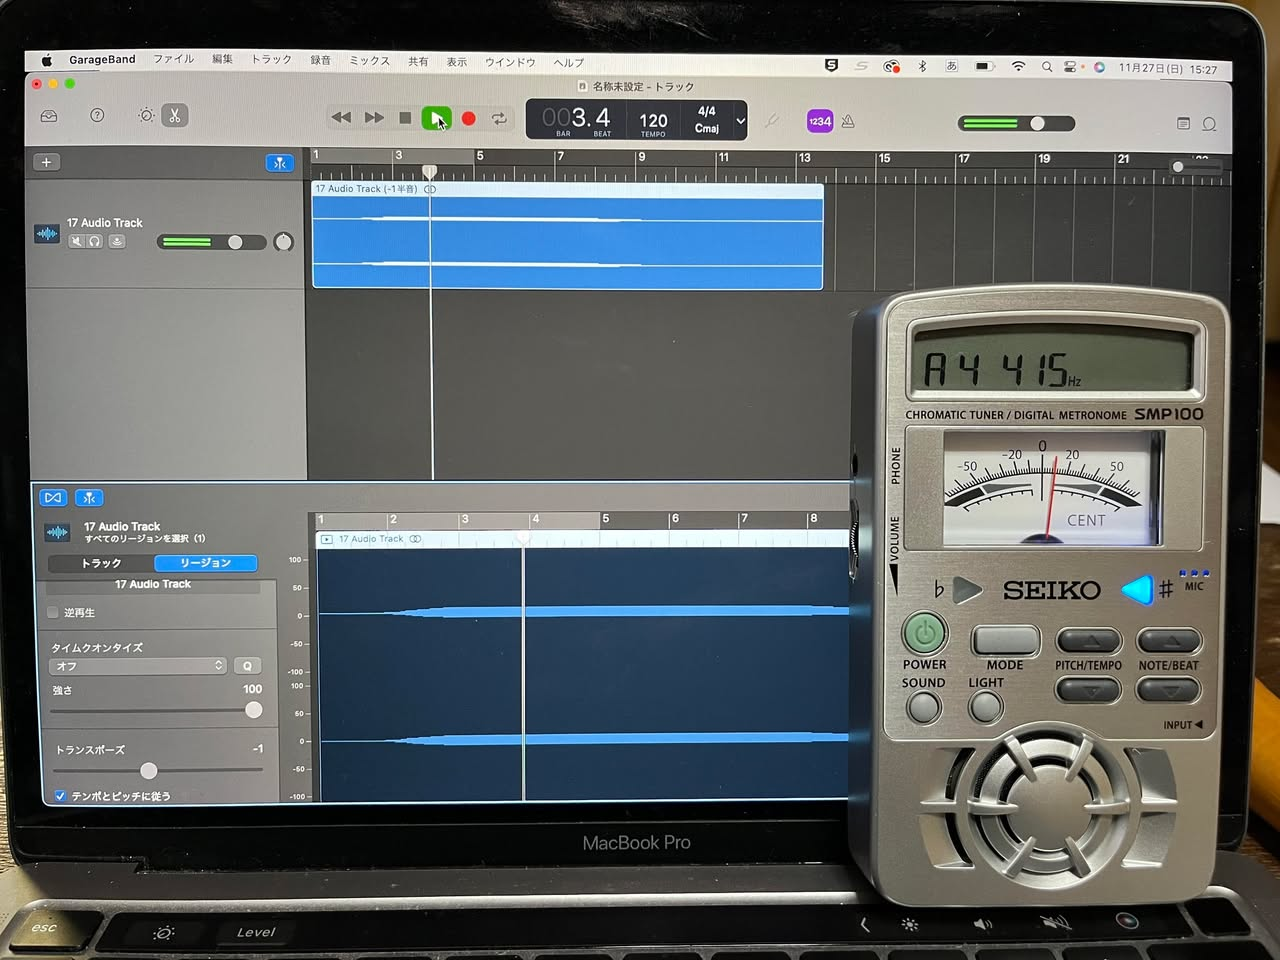
\includegraphics[width=\linewidth]{pictures/2022/11/20221127_140044_001.jpg}
\end{minipage}
\end{center}

\subsection*{2022年11月30日 10:04}
\addcontentsline{toc}{subsection}{2022年11月30日 10:04}

おめでとう。

\subsection*{2022年11月30日 20:20}
\addcontentsline{toc}{subsection}{2022年11月30日 20:20}

楽譜を書く時に使う道具は、人それぞれ好みがあるんでしょうね。万年筆で手書きするのが一番良いと言う方もいらっしゃるかもしれませんが、私はLilyPond(\url{https://lilypond.org/index.html})という楽譜清書用のプログラムを愛用しています。

添付は、Mac 上のEmacs エディタでLilyPondの文法による楽譜の記述、編集をし、それをコンパイルして、PDF を生成している様子です。（PDFの表示にはSkimというプログラムを使っています。）

ここで書いてみている楽譜は、広く知られているJ.S.Bachのシシリアーナです。私は、後で間違いを見つけた時に直しやすくなる様に、右の楽譜の1小節を、左のソース・テキストの1行に対応させて記述することにしています。

最初の2小節の音符だけなら次の通りです。

d8. es16 d8 d g es

c2.

(スラー)を付けると

d8.( es16 d8) d( g es)

c2.

スタッカート(-.)と強弱のp(\textbackslash\{\}p)を付記すると

d8.\textbackslash\{\}p-.( es16-. d8-.) d( g es)

c2.

実際に楽譜の入力作業をしていると、この曲のアーティキュレーションの指定のいろいろ細かい所に気づかされます。（元ネタはBreitkopf版）例えば、スラーとスタッカートの両方が書かれている部分が何ヶ所もあります。この表情、よくあることではありますが、その部分（気持ちはよく分かるのですが）さて具体的にどう吹いたものでしょうか？（少なくとも「単なるスラーではないし、かつ、単なるスタッカートでもない」という意味なのは確かです。また、スラーだけの部分とは「吹き分けたい」所です）困った。でも、これはよくあるアーティキュレーションなのでしょう。JJQuantz大先生の御本を見ると、タンギングの部分で次のように仰っています。（なぜchestが出てくるのかと言うと、タンギングで同じ音の繰り返しを吹く様な譜例になっているからです。with chest action などは現代のメソッドでは異なるのかもしれません）

If a slur is found above notes which are repeated , they must be expressed by exhalation, with chest action.

If, however, dots also stand above such notes , the notes must be expressed much more sharply, and, so to speak, articulated from the chest.

「スラーだけでなくて、ドットも一緒に付いていたら、少しシャープに吹けよ」と仰っているだけ、でしょうか。

また、曲の最終小節への入り方ですが、トリルしようとすると指の動きが困ったことになります（トラヴェルソの場合です）これもJJQuantz先生の御本を参照しますと、トリルの譜例の部分ですが、次の通りです。

The appoggiatura F before E will be transformed into F sharp if the fifth finger is raised too high. Similarly, the D sharp will be transformed into E , the C into C sharp , the B flat into B , the A flat into A , and the A into B flat , whether they appear in the high register or in the low one.

「B flat は、Bに移行して」トリルせよ、と仰っている様な気がします。（この時代のトリルは、多少音痴に聞こえても、それを許容する所があったのか？その音を楽しんだ？のか）

上記いずれの引用も、譜例への参照を省略しているので、何を言っているのか分かりにくいかもしれません。必要に応じて原著(\url{https://books.google.co.jp/books/about/On_Playing_the_Flute.html?id=K--ZaCLuVGAC&redir_esc=y})を参照してくださいませ。

\#LilyPond \#emacs \#JJQuantz \#traverso \#楽譜清書

\paragraph{写真}
\begin{center}
\begin{minipage}{0.70\linewidth}
\centering
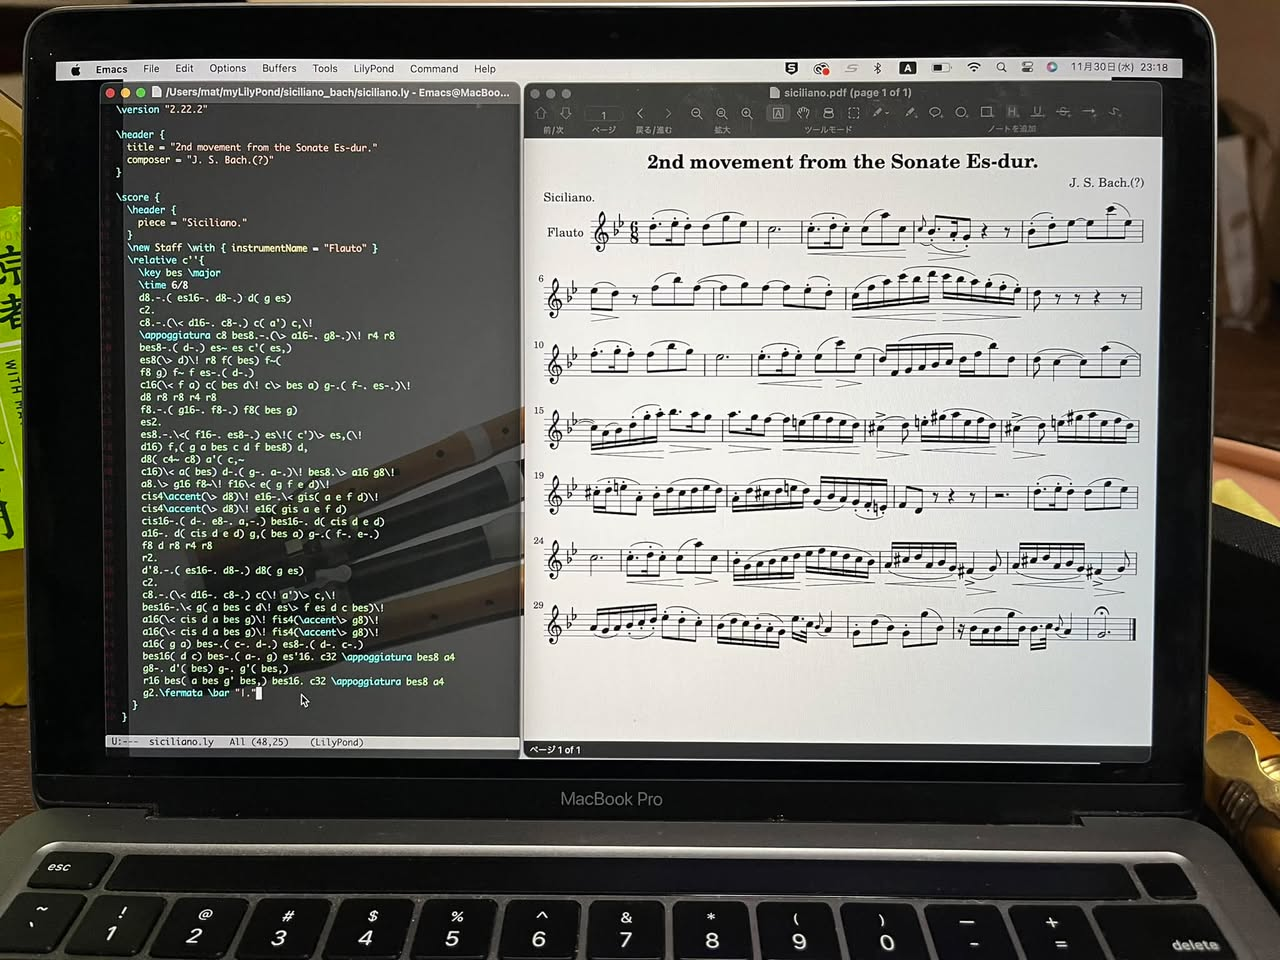
\includegraphics[width=\linewidth]{pictures/2022/11/20221130_202019_001.jpg}
\end{minipage}
\end{center}

\section{12月}

\subsection*{2022年12月04日 12:44}
\addcontentsline{toc}{subsection}{2022年12月04日 12:44}

\url{https://youtu.be/8qaAbFVhjRs}

もとの曲は、S.L.Weissによるlute組曲第５番ト長調です。

luteの曲ですから、Guitarに移して演奏されるのはあり得る事なのですが、ここで私が気にしているのは、かのバルトルド・クイケン氏がトラヴェルソ用に編曲して演奏しているCDです。

私がこの曲を最初に耳にした時には、まるでトラヴェルソの曲かと思わせる感じがしましたので、Quantzの曲にあったかな？Braunか？Telemannてことある？などと、冒頭の数小節を思い出しながら、あれこれ楽譜をひっくり返してみましたが見つからず、ずっと気にしていました。しかしCDを手にしてようやくバルト氏の編曲だと分かったというわけです。

バルト氏は組曲の全曲を移されていますが、その編曲譜を見つける事はできませんでした。そこで、第1曲目のPreludeだけでも楽譜に落とし込んで（演奏して）みようと思い立ちました。しかしバルト氏の演奏を聞いていくと「Weissにインスパイアされて作曲してしまいました」と言わんばかりのアレンジ。ついて行くことができず、Guitar編を元に楽譜にしていくことに方針を変更。Guitar編を聞きながら楽譜を書いて行くうち、これはGuitar編の楽譜を手に入れた方が早そうだと気づき、結局楽譜作りは頓挫したと言う顛末です。お粗末とほほ

Guitar編はこれ(PreludeとAllemande)

\url{https://youtu.be/rUPzpwPymMA}

元のluteの曲はこちら

\url{https://youtu.be/S4msa-MRkoI}

\url{https://youtu.be/9dpuVMdUutM}

\#lute \#Weiss \#Barthold \#Kuijken \#traverso \#リュート \#ヴァイス \#バルト \#クイケン \#トラヴェルソ

\paragraph{リンク}
\url{https://youtu.be/8qaAbFVhjRs}

\subsection*{2022年12月09日 17:59}
\addcontentsline{toc}{subsection}{2022年12月09日 17:59}

新年度に入ると、すぐにやらなければならないのは時間割の編成。県内でも最大規模の学校なので大変です。中でも「実習」は、複数のショップをローテーションして展開するため、複数の教員を担当者としてエントリーさせる必要があります。(TTでも同じことが起きます)その時担当者の名前を1人ずつキーボードから入力しようとすると困ったことになります。梯子「髙」や「齊」藤さんなど、ややこしい漢字が多いこともあって、誤って入力すると別人として処理されてしまいます。

そこで、教員名簿は1つだけExcelシート上に置く事にして、そこから読み出しては実習担当者の文字列を生成する、データ入力支援プログラムを用意してみました。（教務主任はExcelのマクロで作成してほしい様子でしたが、私はExcelのマクロやVBなどは大嫌い！Excelはテストの点数の合計、平均、分散、標準偏差（Z値）などを計算する電卓の代わりでいいのです）比較的得意？なJavaで（以前JaveでExcelを読み書きした経験もあったので）書きはじめることにしました。短いプログラムですが（次年度に、私はここで勤務していないつもりですので）大げさなものは作りたくありません。もし使わないのなら1人1人個別に入力すればいいじゃないか、という程度の感覚で作ってみたものです。

教員は全部で100名程おりますので、全員を並べてそこから選ぶというのは神経衰弱のゲームをするようなもの（苦痛）です。そこで、画面下に並べた3つのコンボボックスで、左から順に「普通教科か工業科か」を選び、真ん中のコンボボックスでは「担当教科(専門学科)」を選び、右端のコンボボックスで、そこまでに絞り込まれた教員の名前の中から選択させ、そこで選択された名前を真ん中のテキスト・フィールドに並べていくというものです。画面上部に並ぶ3つのボタンの左端は、テキスト・フィールドにエントリーされたメンバー文字列をクリアする「Clear」ボタン。真ん中の「BackSpace」は最後にエントリーされた（最も右端の)メンバーを削除するボタン。3番目（右端）の「Copy」は、現在テキスト・フィールドにエントリーされている文字列をクリップボードにコピーするためのボタンです。コピーがすめば、その文字列が必要になる場所でペーストすればよいという訳です。

この程度のプログラムなら、およそ一晩で完成させることができるのですが、これを学校のPCに導入するとなると、おそらくJRE環境を整える所からやり始める事になるんでしょうね。(おっと、Entryのスペルが間違っとるな)

\paragraph{写真}
\begin{center}
\begin{minipage}{0.70\linewidth}
\centering
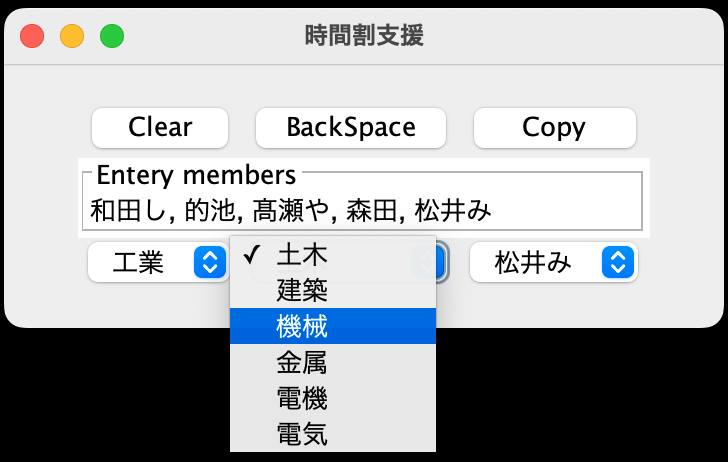
\includegraphics[width=\linewidth]{pictures/2022/12/20221209_175953_001.jpg}
\end{minipage}
\end{center}

\subsection*{2022年12月13日 23:54}
\addcontentsline{toc}{subsection}{2022年12月13日 23:54}

\url{https://github.com/smat1957/pendulum_python}

ランダウとリフシッツによって著された理論物理学教程の「力学」（←名著として誉れ高い）第1章の章末問題を解いてみた。（正解になっている事は保証できない）また、解いた結果をアニメーションにする処理をPythonで書いてみた。（それらしい動きをしているから正解なのかもしれない）

（1）普通の単振子

（2）二重振子（問1）

（3）支点が水平方向に可動な単振子（問2）

（4）支点が円周上を周回している単振子（問3a）

（5）支点が鉛直方向に振動している単振子（問3c）

（6）支点が水平方向に振動している単振子（問3b）

比較的面白いのは(3)でしょうか。支点の質量を大きくして試すと(1)に近づくのが分かります。実際解析的に出てきた結果の式の形からも同じこと（支点の質量→∞に対して、支点の変位→0 で(1)の式に）が予想されます。まあ現象としては当然というか、言われてみれば普通の話なんですけど。また(4)(5)(6)は、一見ややこしそうに見えて実はどれも一緒。支点がもっと複雑に（例えば正弦波上の1周期を往復しているとか☜あまり複雑とも思えないけど）動いたとしても同じ事かと思います。

読んでみようと思う人はあまりいないと思うけど、GitHubへのリンクを置いておきます。srcフォルダにはPythonプログラムとその実行結果であるアニメーションGIFを、readmeフォルダには問題を解析的に解いた手順を書いたPDFとそのTeXのソースを置いています。

\#ランダウ \#リフシッツ \#理論物理学教程 \#力学  \#SHM \#SimpleHarmonicMotion \#単振動 \#Python \#GitHub \#TeX

\paragraph{リンク}
\url{https://github.com/smat1957/pendulum_python}

\subsection*{2022年12月21日 15:29}
\addcontentsline{toc}{subsection}{2022年12月21日 15:29}

\url{https://youtu.be/EMlM6QTzJo0}

↑これって許される事なのでしょうか？

真似をして添付のようなCode(僅か7行)を書いて試してみました。

何事も無かったかのようにダウンロードできました。

でも、やっぱりこれって使っちゃダメなプログラムなんじゃないか？

（自分がアップした動画に限定して使用可という事になるかな）

\paragraph{写真}
\begin{center}
\begin{minipage}{0.70\linewidth}
\centering
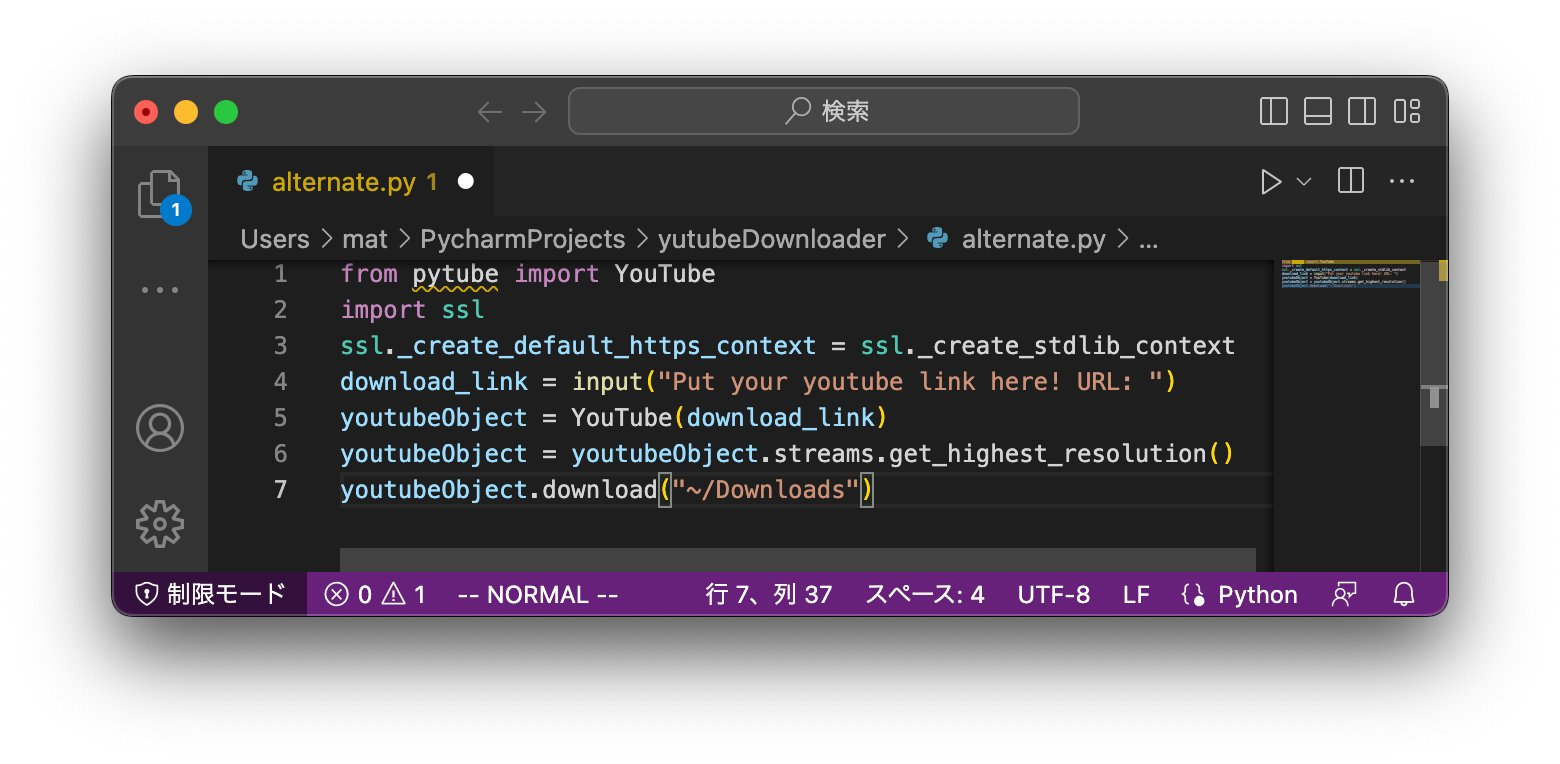
\includegraphics[width=\linewidth]{pictures/2022/12/20221221_152944_001.jpg}
\end{minipage}
\end{center}


\end{document}
